\section{Auswertung}
\label{sec:Auswertung}
\subsection{Geiger-Müller Charakteristik}
Die Daten zur Untersuchung der Geiger-Müller Charakteristik befinden sich in Tab. \ref{tab:charakteristik}.
\begin{table}
    \centering
    \begin{tabular}{ccc}
    \toprule
    $U \,/\, \si{\volt}$ & $N \,/\, \si{\frac{Imp}{60 \second}}$ & $I \,/\, \si{\micro \ampere}$ \\
    \midrule
    320 & 9672 \\
    330 & 9689 \\
    340 & 9580 \\
    350 & 9837 & 0.3 \\
    360 & 9886 \\
    370 & 10041 \\
    380 & 9996 \\
    390 & 9943 \\
    400 & 9995 & 0.4 \\
    410 & 9980 \\
    420 & 9986 \\
    430 & 9960 \\
    440 & 10219 \\
    450 & 10264 & 0.7\\
    460 & 10174 \\
    470 & 10035 \\
    480 & 10350 \\
    490 & 10290 \\
    500 & 10151 & 0.8 \\
    510 & 10110 \\
    \bottomrule
    \end{tabular}
    \begin{tabular}{ccc}
    \toprule
    $U \,/\, \si{\volt}$ & $N \,/\, \si{\frac{Imp}{60 \second}}$ & $I \,/\, \si{\micro \ampere}$ \\
    \midrule
    520 & 10255 \\
    530 & 10151 \\
    540 & 10351 \\
    550 & 10184 & 1.0 \\
    560 & 10137 \\
    570 & 10186 \\
    580 & 10171 \\
    590 & 10171 \\
    600 & 10253 & 1.3 \\
    610 & 10368 \\
    620 & 10365 \\
    630 & 10224 \\
    640 & 10338 \\
    650 & 10493 & 1.4\\
    660 & 10467 \\
    670 & 10640 \\
    680 & 10939 \\
    690 & 11159 \\
    700 & 11547 & 1.8 \\
        &       \\
    \bottomrule
    \end{tabular}
    \caption{Anzahl der Zerfälle $N$ pro $\SI{60}{\second}$ und der Zählrohrstrom $I$ in Abhängigkeit der Spannung $U$.}
    \label{tab:charakteristik}
\end{table}
Der Messfehler für die Impulse $N$ ist nach $\Delta N = \sqrt{N}$ gegeben.
Die Fehler werden im weiteren mithilfe der Bibliothek \glqq uncertainties\grqq \cite{uncertainties} verrechnet.
Werden die gemessenen Impulse durch die Integrationszeit $t = \SI{60}{\second}$  geteilt, ergeben sich die Impulse pro Sekunde.
Die gemessenen Zerfälle pro Sekunde sind in Abb. \ref{fig:char_plot} graphisch dargestellt.
\begin{figure}
    \centering
    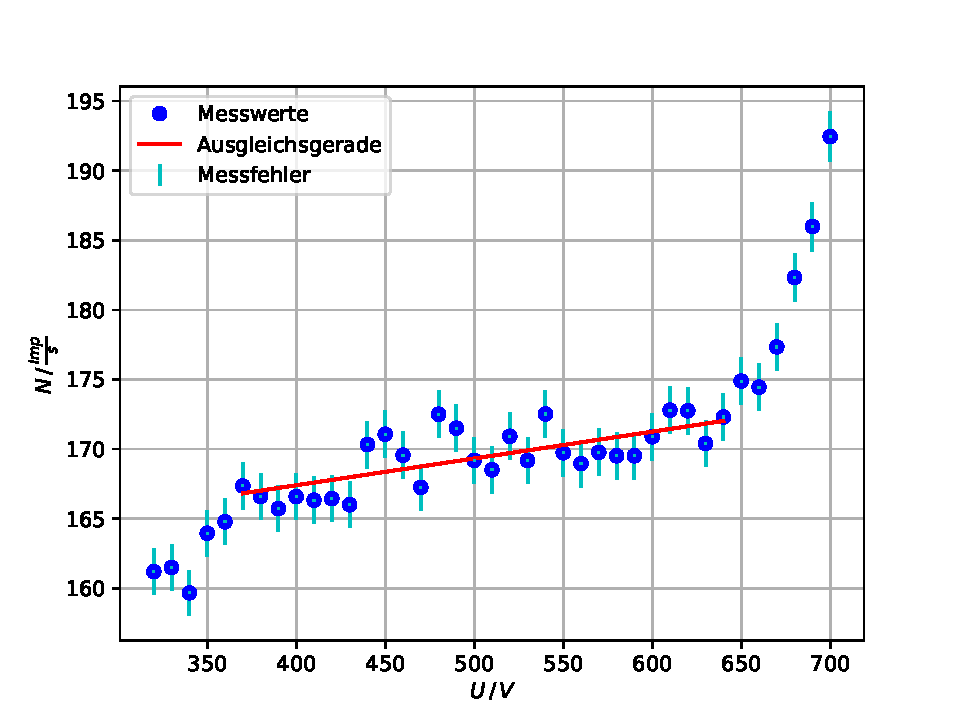
\includegraphics[width=0.8\textwidth]{content/data/charakteristik.pdf}
    \caption{Anzahl der Zerfälle $N$ pro Sekunde mit zugehörigem Fehler in Abhängigkeit der Spannung $U$. Das Plateau wird mit einer linearen Ausgleichsrechnung angenähert. \cite{matplotlib} \cite{scipy} \cite{uncertainties} \cite{numpy}}
    \label{fig:char_plot}
\end{figure}
Das Plateau beginnt bei $U_1 = \SI{370}{\volt}$ und endet bei $U_2 = \SI{640}{\volt}$.
Eine lineare Ausgleichsrechnung
\begin{equation}
    N(U) = a \cdot U + b
\end{equation}
für das Plateau ergibt folgende Parameter:
\begin{align*}
    a = \SI{0.019(4)}{\frac{Imp}{\volt \cdot \second}} \\
    b = \SI{159.7(19)}{\frac{Imp}{s}}
\end{align*}
Die Plateau-Steigung pro $\SI{100}{\volt}$ beträgt
\begin{equation}
    P = \frac{N(\SI{100}{\volt}) - b}{b} = \SI{1.21(23)}{\frac{\percent}{100 \volt}} .
    \label{eqn:plateau_steigung}
\end{equation}
\FloatBarrier

\subsection{Bestimmung der Totzeit}
\label{sec:totzeit}
Zur Bestimmung der Totzeit mithilfe der Zwei-Quellen-Methode ergeben sich folgende Zählraten:
\begin{align*}
    N_1 = \SI{96041}{\frac{Imp}{120 \second}} \\
    N_{1+2} = \SI{158479}{\frac{Imp}{120 \second}} \\
    N_2 = \SI{76518}{\frac{Imp}{120 \second}}
\end{align*}
Nach der Näherung \eqref{eqn:totzeit} ergibt sich die Totzeit
\begin{equation}
    T = \SI{115(4)}{\micro\second} .
\end{equation}
Die Näherung ist gültig, da die folgenden Produkte
\begin{align*}
    T^2 N_1^2 = \SI{0.0085(7)}{{Imp}^2} \\
    T^2 N_{1+2}^2 = \SI{0.0054(4)}{{Imp}^2} \\
    T^2 N_2^2 = \SI{0.0230(16)}{{Imp}^2}
\end{align*}
deutlich kleiner als 1 sind.
\\
Als nächstes wird die Totzeit mit dem Oszilloskop in Abb. \ref{fig:oszi} bestimmt.
\begin{figure}
    \centering
    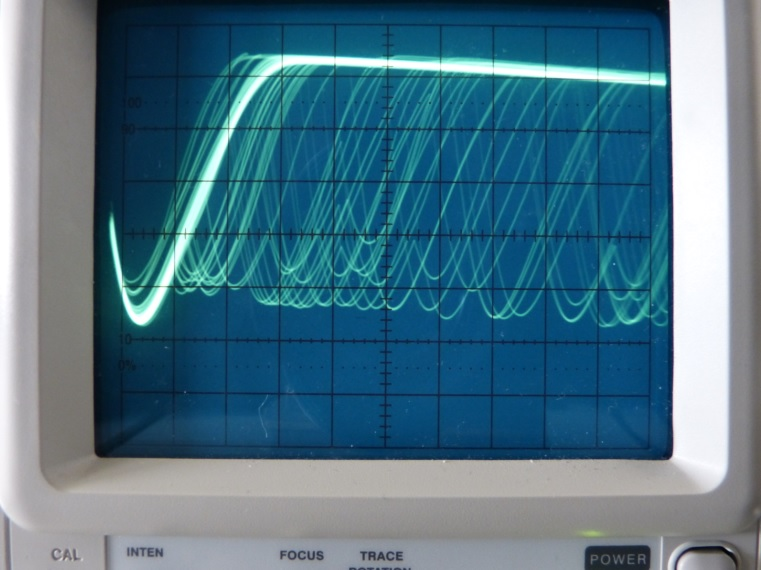
\includegraphics[width=0.8\textwidth]{content/data/oszi.jpg}
    \caption{Aufnahme eines Oszilloskop. Die Zeitachse ist in $\SI{100}{\micro\second \,/\, DIV}$ unterteilt. \cite[2]{hinweise}}
    \label{fig:oszi}
\end{figure}
Die Totzeit beträgt in etwa
\begin{equation}
    T_\text{Oszi} = \SI{100(100)}{\micro\second} .
\end{equation}
\FloatBarrier

\subsection{Bestimmung des Zählrohrstroms}
\label{sec:zaehlstrom}
Der gemessene Zählrohrstrom ist in Tab. \ref{tab:charakteristik} zu sehen.
Der Zählrohrstrom $I$ hat wegen der Ablesegenauigkeit den Fehler $\Delta I = \SI{0.05}{\micro \ampere}$.
In Tab. \ref{tab:zahl_z} befinden sich die Zahlen $Z$ der freigesetzten Ladungen pro einfallende Teilchen \eqref{eqn:Z}.
Die zur Berechnung notwendige Elementarladung wird der Literatur entnommen. \cite{konst}
\\
\begin{table}
    \centering
    \begin{tabular}{cc}
        \toprule
        $I \,/\, \si{\micro \ampere}$ & $Z \,/\, 10^9$ \\
        \midrule
        $\SI{0.30(5)}{}$ & $\SI{11.42(191)}{}$ \\
        $\SI{0.40(5)}{}$ & $\SI{14.99(188)}{}$ \\
        $\SI{0.70(5)}{}$ & $\SI{25.54(184)}{}$ \\
        $\SI{0.80(5)}{}$ & $\SI{29.51(187)}{}$ \\
        $\SI{1.00(5)}{}$ & $\SI{36.77(187)}{}$ \\
        $\SI{1.30(5)}{}$ & $\SI{47.48(189)}{}$ \\
        $\SI{1.40(5)}{}$ & $\SI{49.97(185)}{}$ \\
        $\SI{1.80(5)}{}$ & $\SI{58.38(171)}{}$ \\
        \bottomrule
    \end{tabular}
    \caption{Die berrechnete Zahl $Z$ und der gemessene Zählrohrstrom $I$ aufgelistet.}
    \label{tab:zahl_z}
\end{table}
In der Abb. \ref{fig:zahl_z} sind die Zahlen Z in Abhängigkeit vom Zählrohrstrom $I$ dargestellt.
\begin{figure}
    \centering
    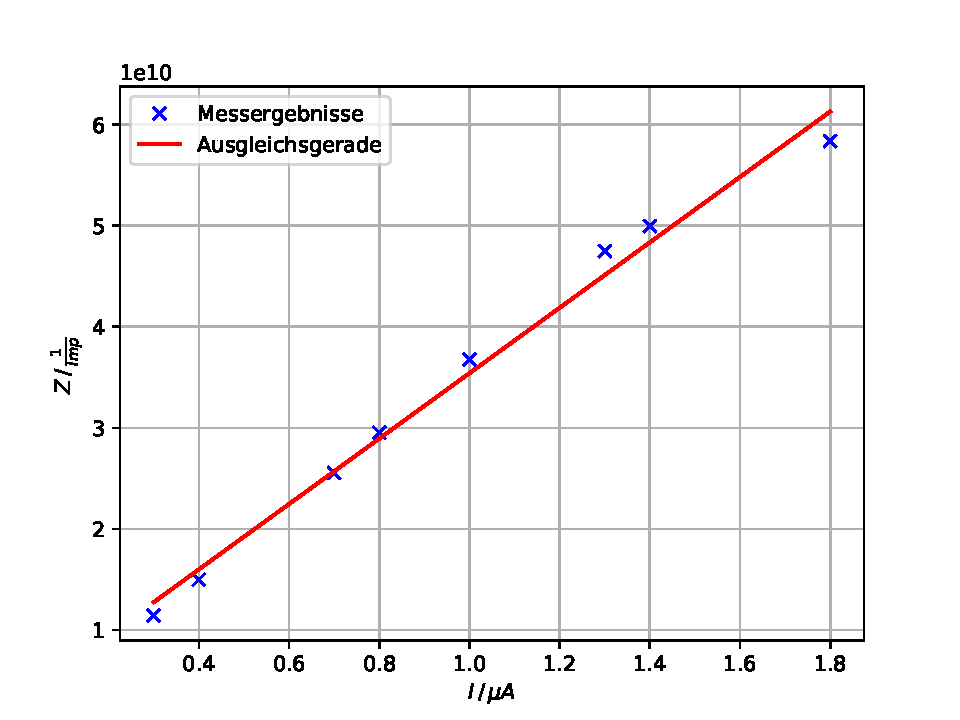
\includegraphics[width=0.7\textwidth]{content/data/zaehlrohrstrom.pdf}
    \caption{Die Zahl $Z$ in Abhängigkeit vom Zählrohrstrom $I$ und eine Ausgleichsgerade. \cite{matplotlib} \cite{scipy} \cite{numpy}}
    \label{fig:zahl_z}
\end{figure}
\FloatBarrier
Eine lineare Ausgleichsrechnung
\begin{equation*}
    Z = I \cdot a + b
\end{equation*}
ergibt folgende Parameter:
\begin{align*}
    a = \SI{3.24(14)e16}{\frac{1}{Imp \cdot \ampere}} \\
    b = \SI{3.0(15)e9}{\frac{1}{Imp}}
\end{align*}